\section{}
% Street performers often use a “gut bucket”, or washtub bass, to produce frequencies near the 
% resonant frequency of the human chest cavity (~10 Hz). This is a crude instrument made from a 
% wire stretched between points B and C. The wire is plucked to create transverse vibrations, and the
% tension in the wire is created by applying a rigid force 𝑃 to rigid member 𝐴𝐷. The instrument uses 
% a steel wire, with a diameter of 2 mm and density of 7800 kg/m3
% .

\textit{Street performers often use a “gut bucket”, or washtub bass, to produce frequencies near the resonant frequency of the human chest cavity (~10 Hz). This is a crude instrument made from a wire stretched between points B and C. The wire is plucked to create transverse vibrations, and the tension in the wire is created by applying a rigid force $P$ to rigid member AD. The instrument uses a steel wire, with a diameter of 2 mm and density of 7800 kg/m$^3$.}

\subsection{}
\textit{(5 pts) Determine the required distance $h$ so that the string has a fundamental frequency of 15 Hz when a force of 15 N is applied to member AD.}
We want the fundamental frequency to be $p = 2\pi f = 94.25$ rad/s. The fundamental frequency of a string is given by
\begin{align}
    p &= \frac{c \pi}{L} \nonumber \\
    &= \frac{\sqrt{\frac{T}{\rho}} \pi}{L} \label{eq:Q1 freq} 
\end{align}
The linear density, $\rho$, of the wire is given by
\begin{align*}
    \rho_{\text{lin}} &= \frac{\pi}{4} d^2 \rho_{\text{steel}} \\
    &= \frac{\pi}{4} (0.002)^2 (7800) \\
    &= 0.0245 \text{ kg/m}
\end{align*}
Next, the free body diagram of the gut bucket is shown in Figure \ref{fig:Q1 FBD}. 
\begin{figure}[h]
    \centering
    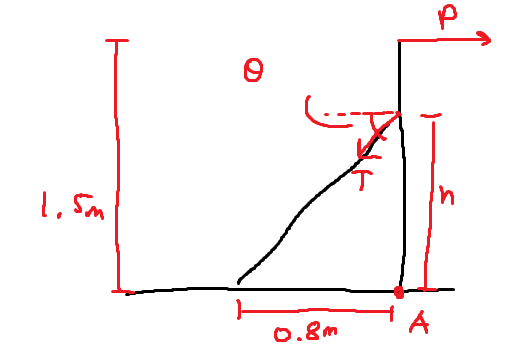
\includegraphics[width=0.5\textwidth]{Questions/Figures/Q1 FBD.png}
    \caption{Free body diagram of the gut bucket}
    \label{fig:Q1 FBD}
\end{figure}
Since the bucket is in equilibrium, take the moment about the pin $A$,
\begin{align*}
    \circlearrowleft \sum M_A &= 0 \\
    &= T h \cos\theta - P (1.5) 
\end{align*}
where $\theta = \tan^{-1} \left(\frac{h}{0.8}\right)$. The tension in the wire is given by
\begin{align*}
    T &= \frac{P (1.5)}{h \cos\left(\tan^{-1} \left(\frac{h}{0.8}\right)\right)} 
\end{align*}
Using the property that 
\begin{align*}
    \cos\left(\tan^{-1} (x)\right) = \frac{1}{\sqrt{1 + x^2}}
\end{align*}
the tension in the wire is given by
\begin{align*}
    T &= \frac{P (1.5) \sqrt{1 + \left(\frac{h}{0.8}\right)^2}}{h} \\
    &= \frac{15 (1.5) \sqrt{1 + \left(\frac{h}{0.8}\right)^2}}{h} \\
    &= \frac{22.5 \sqrt{1 + \left(\frac{h}{0.8}\right)^2}}{h}
\end{align*}
substituting the given values into Eq. (\ref{eq:Q1 freq}),
\begin{align*}
    p &= \frac{\sqrt{\frac{T}{0.0245}} \pi}{\sqrt{(0.8)^2 + h^2}} \\
    94.25 &= \frac{\sqrt{\frac{22.5 \sqrt{1 + \left(\frac{h}{0.8}\right)^2}}{7800h}} \pi}{\sqrt{(0.8)^2 + h^2}} 
\end{align*}
Using MATLAB, 
\begin{verbatim}
syms h
eqn = sqrt(22.5*sqrt((1 + (h/0.8)^2))/(0.0245*h))*pi/sqrt((0.8)^2 + h^2) == 2*pi*15;
sol = vpasolve(eqn, h)

>> sol = 0.99751616990113187949217696874991
\end{verbatim}
Therefore, 
\begin{empheq}[box=\fbox]{align*}
    h &= 0.998 \text{ m}
\end{empheq}

\subsection{}
\textit{For a distance $h$ of 1.2 m, what range of force ($P_1$ to $P_2$) is necessary to produce notes that cover an entire octave from 20 to 40 Hz?}
The fundamental frequency of the string is given by Eq. (\ref{eq:Q1 freq}),
\begin{align*}
    p &= \frac{\sqrt{\frac{T}{\rho}} \pi}{L} \\
   \implies T &= \frac{p^2 \rho L^2}{\pi^2} 
\end{align*}
Calculating $L$ and $\theta$,
\begin{align*}
    L &= \sqrt{(0.8)^2 + (1.2)^2} \\
    &= 1.442 \text{ m} \\
    \theta &= \tan^{-1} \left(\frac{1.2}{0.8}\right) \\
    &= 56.301^\circ
\end{align*}
Recall from the free body diagram that 
\begin{align*}
    P &= \frac{T h \cos\theta}{1.5} \\
    &= \frac{p^2 \rho L^2 h \cos\theta}{1.5 \pi^2} 
\end{align*}
Then for $P_1$ and $P_2$,
\begin{empheq}[box=\fbox]{align*}
    P_1 &= \frac{p_1^2 \rho L^2 h \cos\theta}{1.5 \pi^2} \\
    &= \frac{(2\pi 20)^2 (0.0245) (1.442) (1.2) \cos(56.301)}{1.5 \pi^2} \\
    &= 25.09 \text{ N} \\
    P_2 &= \frac{p_2^2 \rho L^2 h \cos\theta}{1.5 \pi^2} \\
    &= \frac{(2\pi 40)^2 (0.0245) (1.442) (1.2) \cos(56.301)}{1.5 \pi^2} \\
    &= 100.36 \text{ N}
\end{empheq}    